% Created by tikzDevice version 0.12.3 on 2019-09-27 15:50:44
% !TEX encoding = UTF-8 Unicode
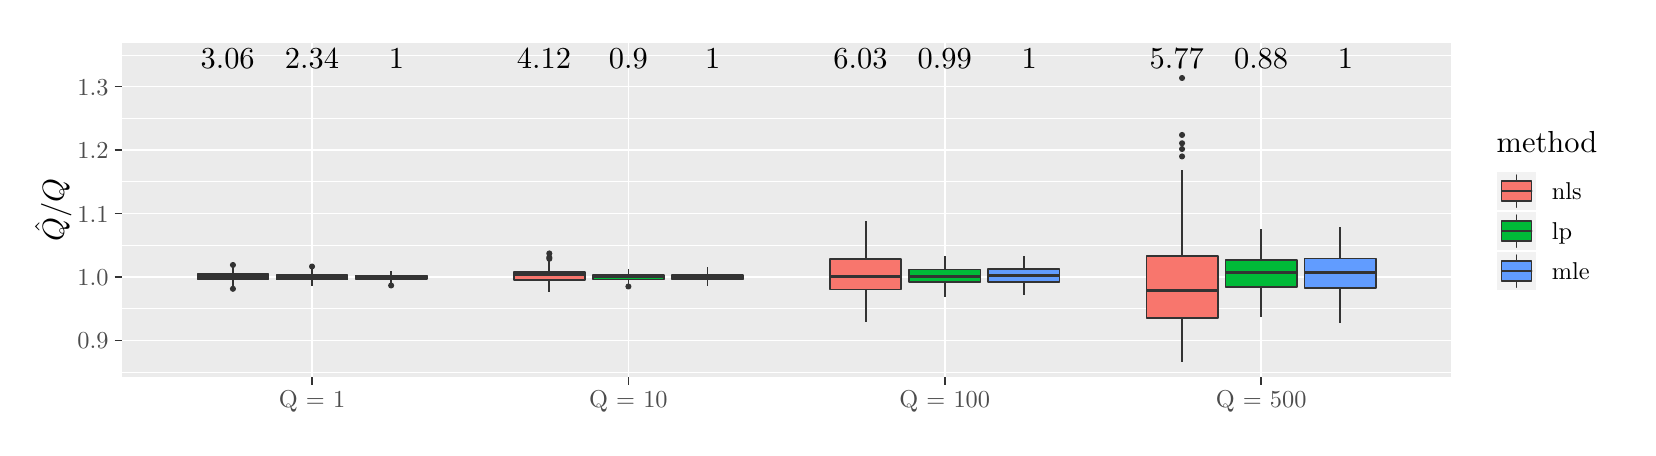
\begin{tikzpicture}[x=1pt,y=1pt]
\definecolor{fillColor}{RGB}{255,255,255}
\path[use as bounding box,fill=fillColor,fill opacity=0.00] (0,0) rectangle (578.16,144.54);
\begin{scope}
\path[clip] (  0.00,  0.00) rectangle (578.16,144.54);
\definecolor{drawColor}{RGB}{255,255,255}
\definecolor{fillColor}{RGB}{255,255,255}

\path[draw=drawColor,line width= 0.6pt,line join=round,line cap=round,fill=fillColor] (  0.00,  0.00) rectangle (578.16,144.54);
\end{scope}
\begin{scope}
\path[clip] ( 34.16, 18.22) rectangle (514.31,139.04);
\definecolor{fillColor}{gray}{0.92}

\path[fill=fillColor] ( 34.16, 18.22) rectangle (514.31,139.04);
\definecolor{drawColor}{RGB}{255,255,255}

\path[draw=drawColor,line width= 0.3pt,line join=round] ( 34.16, 20.01) --
	(514.31, 20.01);

\path[draw=drawColor,line width= 0.3pt,line join=round] ( 34.16, 42.95) --
	(514.31, 42.95);

\path[draw=drawColor,line width= 0.3pt,line join=round] ( 34.16, 65.88) --
	(514.31, 65.88);

\path[draw=drawColor,line width= 0.3pt,line join=round] ( 34.16, 88.82) --
	(514.31, 88.82);

\path[draw=drawColor,line width= 0.3pt,line join=round] ( 34.16,111.75) --
	(514.31,111.75);

\path[draw=drawColor,line width= 0.3pt,line join=round] ( 34.16,134.69) --
	(514.31,134.69);

\path[draw=drawColor,line width= 0.6pt,line join=round] ( 34.16, 31.48) --
	(514.31, 31.48);

\path[draw=drawColor,line width= 0.6pt,line join=round] ( 34.16, 54.41) --
	(514.31, 54.41);

\path[draw=drawColor,line width= 0.6pt,line join=round] ( 34.16, 77.35) --
	(514.31, 77.35);

\path[draw=drawColor,line width= 0.6pt,line join=round] ( 34.16,100.28) --
	(514.31,100.28);

\path[draw=drawColor,line width= 0.6pt,line join=round] ( 34.16,123.22) --
	(514.31,123.22);

\path[draw=drawColor,line width= 0.6pt,line join=round] (102.75, 18.22) --
	(102.75,139.04);

\path[draw=drawColor,line width= 0.6pt,line join=round] (217.07, 18.22) --
	(217.07,139.04);

\path[draw=drawColor,line width= 0.6pt,line join=round] (331.39, 18.22) --
	(331.39,139.04);

\path[draw=drawColor,line width= 0.6pt,line join=round] (445.71, 18.22) --
	(445.71,139.04);
\definecolor{drawColor}{gray}{0.20}
\definecolor{fillColor}{gray}{0.20}

\path[draw=drawColor,line width= 0.4pt,line join=round,line cap=round,fill=fillColor] ( 74.17, 58.79) circle (  0.89);

\path[draw=drawColor,line width= 0.4pt,line join=round,line cap=round,fill=fillColor] ( 74.17, 50.18) circle (  0.89);

\path[draw=drawColor,line width= 0.6pt,line join=round] ( 74.17, 55.56) -- ( 74.17, 58.30);

\path[draw=drawColor,line width= 0.6pt,line join=round] ( 74.17, 53.57) -- ( 74.17, 50.81);
\definecolor{fillColor}{RGB}{248,118,109}

\path[draw=drawColor,line width= 0.6pt,line join=round,line cap=round,fill=fillColor] ( 61.31, 55.56) --
	( 61.31, 53.57) --
	( 87.03, 53.57) --
	( 87.03, 55.56) --
	( 61.31, 55.56) --
	cycle;

\path[draw=drawColor,line width= 1.1pt,line join=round] ( 61.31, 54.45) -- ( 87.03, 54.45);
\definecolor{fillColor}{gray}{0.20}

\path[draw=drawColor,line width= 0.4pt,line join=round,line cap=round,fill=fillColor] (102.75, 58.24) circle (  0.89);

\path[draw=drawColor,line width= 0.6pt,line join=round] (102.75, 55.21) -- (102.75, 57.52);

\path[draw=drawColor,line width= 0.6pt,line join=round] (102.75, 53.50) -- (102.75, 51.09);
\definecolor{fillColor}{RGB}{0,186,56}

\path[draw=drawColor,line width= 0.6pt,line join=round,line cap=round,fill=fillColor] ( 89.89, 55.21) --
	( 89.89, 53.50) --
	(115.61, 53.50) --
	(115.61, 55.21) --
	( 89.89, 55.21) --
	cycle;

\path[draw=drawColor,line width= 1.1pt,line join=round] ( 89.89, 54.35) -- (115.61, 54.35);
\definecolor{fillColor}{gray}{0.20}

\path[draw=drawColor,line width= 0.4pt,line join=round,line cap=round,fill=fillColor] (131.33, 51.38) circle (  0.89);

\path[draw=drawColor,line width= 0.6pt,line join=round] (131.33, 54.99) -- (131.33, 56.71);

\path[draw=drawColor,line width= 0.6pt,line join=round] (131.33, 53.79) -- (131.33, 52.34);
\definecolor{fillColor}{RGB}{97,156,255}

\path[draw=drawColor,line width= 0.6pt,line join=round,line cap=round,fill=fillColor] (118.47, 54.99) --
	(118.47, 53.79) --
	(144.19, 53.79) --
	(144.19, 54.99) --
	(118.47, 54.99) --
	cycle;

\path[draw=drawColor,line width= 1.1pt,line join=round] (118.47, 54.41) -- (144.19, 54.41);
\definecolor{fillColor}{gray}{0.20}

\path[draw=drawColor,line width= 0.4pt,line join=round,line cap=round,fill=fillColor] (188.49, 61.55) circle (  0.89);

\path[draw=drawColor,line width= 0.4pt,line join=round,line cap=round,fill=fillColor] (188.49, 61.03) circle (  0.89);

\path[draw=drawColor,line width= 0.4pt,line join=round,line cap=round,fill=fillColor] (188.49, 62.95) circle (  0.89);

\path[draw=drawColor,line width= 0.6pt,line join=round] (188.49, 56.30) -- (188.49, 60.50);

\path[draw=drawColor,line width= 0.6pt,line join=round] (188.49, 53.26) -- (188.49, 48.91);
\definecolor{fillColor}{RGB}{248,118,109}

\path[draw=drawColor,line width= 0.6pt,line join=round,line cap=round,fill=fillColor] (175.63, 56.30) --
	(175.63, 53.26) --
	(201.35, 53.26) --
	(201.35, 56.30) --
	(175.63, 56.30) --
	cycle;

\path[draw=drawColor,line width= 1.1pt,line join=round] (175.63, 55.18) -- (201.35, 55.18);
\definecolor{fillColor}{gray}{0.20}

\path[draw=drawColor,line width= 0.4pt,line join=round,line cap=round,fill=fillColor] (217.07, 51.01) circle (  0.89);

\path[draw=drawColor,line width= 0.6pt,line join=round] (217.07, 55.27) -- (217.07, 57.39);

\path[draw=drawColor,line width= 0.6pt,line join=round] (217.07, 53.59) -- (217.07, 51.69);
\definecolor{fillColor}{RGB}{0,186,56}

\path[draw=drawColor,line width= 0.6pt,line join=round,line cap=round,fill=fillColor] (204.21, 55.27) --
	(204.21, 53.59) --
	(229.93, 53.59) --
	(229.93, 55.27) --
	(204.21, 55.27) --
	cycle;

\path[draw=drawColor,line width= 1.1pt,line join=round] (204.21, 54.51) -- (229.93, 54.51);

\path[draw=drawColor,line width= 0.6pt,line join=round] (245.65, 55.27) -- (245.65, 57.92);

\path[draw=drawColor,line width= 0.6pt,line join=round] (245.65, 53.49) -- (245.65, 51.14);
\definecolor{fillColor}{RGB}{97,156,255}

\path[draw=drawColor,line width= 0.6pt,line join=round,line cap=round,fill=fillColor] (232.79, 55.27) --
	(232.79, 53.49) --
	(258.51, 53.49) --
	(258.51, 55.27) --
	(232.79, 55.27) --
	cycle;

\path[draw=drawColor,line width= 1.1pt,line join=round] (232.79, 54.37) -- (258.51, 54.37);

\path[draw=drawColor,line width= 0.6pt,line join=round] (302.81, 60.83) -- (302.81, 74.69);

\path[draw=drawColor,line width= 0.6pt,line join=round] (302.81, 49.91) -- (302.81, 38.19);
\definecolor{fillColor}{RGB}{248,118,109}

\path[draw=drawColor,line width= 0.6pt,line join=round,line cap=round,fill=fillColor] (289.95, 60.83) --
	(289.95, 49.91) --
	(315.67, 49.91) --
	(315.67, 60.83) --
	(289.95, 60.83) --
	cycle;

\path[draw=drawColor,line width= 1.1pt,line join=round] (289.95, 54.53) -- (315.67, 54.53);

\path[draw=drawColor,line width= 0.6pt,line join=round] (331.39, 57.12) -- (331.39, 62.10);

\path[draw=drawColor,line width= 0.6pt,line join=round] (331.39, 52.59) -- (331.39, 47.06);
\definecolor{fillColor}{RGB}{0,186,56}

\path[draw=drawColor,line width= 0.6pt,line join=round,line cap=round,fill=fillColor] (318.53, 57.12) --
	(318.53, 52.59) --
	(344.25, 52.59) --
	(344.25, 57.12) --
	(318.53, 57.12) --
	cycle;

\path[draw=drawColor,line width= 1.1pt,line join=round] (318.53, 54.70) -- (344.25, 54.70);

\path[draw=drawColor,line width= 0.6pt,line join=round] (359.97, 57.44) -- (359.97, 61.94);

\path[draw=drawColor,line width= 0.6pt,line join=round] (359.97, 52.57) -- (359.97, 47.79);
\definecolor{fillColor}{RGB}{97,156,255}

\path[draw=drawColor,line width= 0.6pt,line join=round,line cap=round,fill=fillColor] (347.11, 57.44) --
	(347.11, 52.57) --
	(372.83, 52.57) --
	(372.83, 57.44) --
	(347.11, 57.44) --
	cycle;

\path[draw=drawColor,line width= 1.1pt,line join=round] (347.11, 54.85) -- (372.83, 54.85);
\definecolor{fillColor}{gray}{0.20}

\path[draw=drawColor,line width= 0.4pt,line join=round,line cap=round,fill=fillColor] (417.13,102.78) circle (  0.89);

\path[draw=drawColor,line width= 0.4pt,line join=round,line cap=round,fill=fillColor] (417.13,100.69) circle (  0.89);

\path[draw=drawColor,line width= 0.4pt,line join=round,line cap=round,fill=fillColor] (417.13, 98.00) circle (  0.89);

\path[draw=drawColor,line width= 0.4pt,line join=round,line cap=round,fill=fillColor] (417.13,105.77) circle (  0.89);

\path[draw=drawColor,line width= 0.4pt,line join=round,line cap=round,fill=fillColor] (417.13,126.35) circle (  0.89);

\path[draw=drawColor,line width= 0.6pt,line join=round] (417.13, 62.13) -- (417.13, 92.93);

\path[draw=drawColor,line width= 0.6pt,line join=round] (417.13, 39.58) -- (417.13, 23.71);
\definecolor{fillColor}{RGB}{248,118,109}

\path[draw=drawColor,line width= 0.6pt,line join=round,line cap=round,fill=fillColor] (404.27, 62.13) --
	(404.27, 39.58) --
	(430.00, 39.58) --
	(430.00, 62.13) --
	(404.27, 62.13) --
	cycle;

\path[draw=drawColor,line width= 1.1pt,line join=round] (404.27, 49.62) -- (430.00, 49.62);

\path[draw=drawColor,line width= 0.6pt,line join=round] (445.71, 60.50) -- (445.71, 71.88);

\path[draw=drawColor,line width= 0.6pt,line join=round] (445.71, 50.75) -- (445.71, 39.90);
\definecolor{fillColor}{RGB}{0,186,56}

\path[draw=drawColor,line width= 0.6pt,line join=round,line cap=round,fill=fillColor] (432.85, 60.50) --
	(432.85, 50.75) --
	(458.58, 50.75) --
	(458.58, 60.50) --
	(432.85, 60.50) --
	cycle;

\path[draw=drawColor,line width= 1.1pt,line join=round] (432.85, 56.06) -- (458.58, 56.06);

\path[draw=drawColor,line width= 0.6pt,line join=round] (474.29, 61.16) -- (474.29, 72.43);

\path[draw=drawColor,line width= 0.6pt,line join=round] (474.29, 50.38) -- (474.29, 37.96);
\definecolor{fillColor}{RGB}{97,156,255}

\path[draw=drawColor,line width= 0.6pt,line join=round,line cap=round,fill=fillColor] (461.43, 61.16) --
	(461.43, 50.38) --
	(487.16, 50.38) --
	(487.16, 61.16) --
	(461.43, 61.16) --
	cycle;

\path[draw=drawColor,line width= 1.1pt,line join=round] (461.43, 55.90) -- (487.16, 55.90);
\definecolor{drawColor}{RGB}{0,0,0}

\node[text=drawColor,anchor=base,inner sep=0pt, outer sep=0pt, scale=  1.10] at (133.23,129.75) {1};

\node[text=drawColor,anchor=base,inner sep=0pt, outer sep=0pt, scale=  1.10] at (102.75,129.75) {2.34};

\node[text=drawColor,anchor=base,inner sep=0pt, outer sep=0pt, scale=  1.10] at ( 72.26,129.75) {3.06};

\node[text=drawColor,anchor=base,inner sep=0pt, outer sep=0pt, scale=  1.10] at (247.56,129.75) {1};

\node[text=drawColor,anchor=base,inner sep=0pt, outer sep=0pt, scale=  1.10] at (217.07,129.75) {0.9};

\node[text=drawColor,anchor=base,inner sep=0pt, outer sep=0pt, scale=  1.10] at (186.59,129.75) {4.12};

\node[text=drawColor,anchor=base,inner sep=0pt, outer sep=0pt, scale=  1.10] at (361.88,129.75) {1};

\node[text=drawColor,anchor=base,inner sep=0pt, outer sep=0pt, scale=  1.10] at (331.39,129.75) {0.99};

\node[text=drawColor,anchor=base,inner sep=0pt, outer sep=0pt, scale=  1.10] at (300.91,129.75) {6.03};

\node[text=drawColor,anchor=base,inner sep=0pt, outer sep=0pt, scale=  1.10] at (476.20,129.75) {1};

\node[text=drawColor,anchor=base,inner sep=0pt, outer sep=0pt, scale=  1.10] at (445.71,129.75) {0.88};

\node[text=drawColor,anchor=base,inner sep=0pt, outer sep=0pt, scale=  1.10] at (415.23,129.75) {5.77};
\end{scope}
\begin{scope}
\path[clip] (  0.00,  0.00) rectangle (578.16,144.54);
\definecolor{drawColor}{gray}{0.30}

\node[text=drawColor,anchor=base east,inner sep=0pt, outer sep=0pt, scale=  0.88] at ( 29.21, 28.45) {0.9};

\node[text=drawColor,anchor=base east,inner sep=0pt, outer sep=0pt, scale=  0.88] at ( 29.21, 51.38) {1.0};

\node[text=drawColor,anchor=base east,inner sep=0pt, outer sep=0pt, scale=  0.88] at ( 29.21, 74.32) {1.1};

\node[text=drawColor,anchor=base east,inner sep=0pt, outer sep=0pt, scale=  0.88] at ( 29.21, 97.25) {1.2};

\node[text=drawColor,anchor=base east,inner sep=0pt, outer sep=0pt, scale=  0.88] at ( 29.21,120.19) {1.3};
\end{scope}
\begin{scope}
\path[clip] (  0.00,  0.00) rectangle (578.16,144.54);
\definecolor{drawColor}{gray}{0.20}

\path[draw=drawColor,line width= 0.6pt,line join=round] ( 31.41, 31.48) --
	( 34.16, 31.48);

\path[draw=drawColor,line width= 0.6pt,line join=round] ( 31.41, 54.41) --
	( 34.16, 54.41);

\path[draw=drawColor,line width= 0.6pt,line join=round] ( 31.41, 77.35) --
	( 34.16, 77.35);

\path[draw=drawColor,line width= 0.6pt,line join=round] ( 31.41,100.28) --
	( 34.16,100.28);

\path[draw=drawColor,line width= 0.6pt,line join=round] ( 31.41,123.22) --
	( 34.16,123.22);
\end{scope}
\begin{scope}
\path[clip] (  0.00,  0.00) rectangle (578.16,144.54);
\definecolor{drawColor}{gray}{0.20}

\path[draw=drawColor,line width= 0.6pt,line join=round] (102.75, 15.47) --
	(102.75, 18.22);

\path[draw=drawColor,line width= 0.6pt,line join=round] (217.07, 15.47) --
	(217.07, 18.22);

\path[draw=drawColor,line width= 0.6pt,line join=round] (331.39, 15.47) --
	(331.39, 18.22);

\path[draw=drawColor,line width= 0.6pt,line join=round] (445.71, 15.47) --
	(445.71, 18.22);
\end{scope}
\begin{scope}
\path[clip] (  0.00,  0.00) rectangle (578.16,144.54);
\definecolor{drawColor}{gray}{0.30}

\node[text=drawColor,anchor=base,inner sep=0pt, outer sep=0pt, scale=  0.88] at (102.75,  7.21) {Q = 1};

\node[text=drawColor,anchor=base,inner sep=0pt, outer sep=0pt, scale=  0.88] at (217.07,  7.21) {Q = 10};

\node[text=drawColor,anchor=base,inner sep=0pt, outer sep=0pt, scale=  0.88] at (331.39,  7.21) {Q = 100};

\node[text=drawColor,anchor=base,inner sep=0pt, outer sep=0pt, scale=  0.88] at (445.71,  7.21) {Q = 500};
\end{scope}
\begin{scope}
\path[clip] (  0.00,  0.00) rectangle (578.16,144.54);
\definecolor{drawColor}{RGB}{0,0,0}

\node[text=drawColor,rotate= 90.00,anchor=base,inner sep=0pt, outer sep=0pt, scale=  1.10] at ( 13.08, 78.63) {$\hat{Q}/Q$};
\end{scope}
\begin{scope}
\path[clip] (  0.00,  0.00) rectangle (578.16,144.54);
\definecolor{fillColor}{RGB}{255,255,255}

\path[fill=fillColor] (525.31, 43.84) rectangle (572.66,113.42);
\end{scope}
\begin{scope}
\path[clip] (  0.00,  0.00) rectangle (578.16,144.54);
\definecolor{drawColor}{RGB}{0,0,0}

\node[text=drawColor,anchor=base west,inner sep=0pt, outer sep=0pt, scale=  1.10] at (530.81, 99.27) {method};
\end{scope}
\begin{scope}
\path[clip] (  0.00,  0.00) rectangle (578.16,144.54);
\definecolor{drawColor}{RGB}{255,255,255}
\definecolor{fillColor}{gray}{0.95}

\path[draw=drawColor,line width= 0.6pt,line join=round,line cap=round,fill=fillColor] (530.81, 78.25) rectangle (545.26, 92.70);
\end{scope}
\begin{scope}
\path[clip] (  0.00,  0.00) rectangle (578.16,144.54);
\definecolor{drawColor}{gray}{0.20}

\path[draw=drawColor,line width= 0.6pt,line join=round,line cap=round] (538.03, 79.70) --
	(538.03, 81.86);

\path[draw=drawColor,line width= 0.6pt,line join=round,line cap=round] (538.03, 89.09) --
	(538.03, 91.26);
\definecolor{fillColor}{RGB}{248,118,109}

\path[draw=drawColor,line width= 0.6pt,line join=round,line cap=round,fill=fillColor] (532.61, 81.86) rectangle (543.45, 89.09);

\path[draw=drawColor,line width= 0.6pt,line join=round,line cap=round] (532.61, 85.48) --
	(543.45, 85.48);
\end{scope}
\begin{scope}
\path[clip] (  0.00,  0.00) rectangle (578.16,144.54);
\definecolor{drawColor}{RGB}{255,255,255}
\definecolor{fillColor}{gray}{0.95}

\path[draw=drawColor,line width= 0.6pt,line join=round,line cap=round,fill=fillColor] (530.81, 63.80) rectangle (545.26, 78.25);
\end{scope}
\begin{scope}
\path[clip] (  0.00,  0.00) rectangle (578.16,144.54);
\definecolor{drawColor}{gray}{0.20}

\path[draw=drawColor,line width= 0.6pt,line join=round,line cap=round] (538.03, 65.24) --
	(538.03, 67.41);

\path[draw=drawColor,line width= 0.6pt,line join=round,line cap=round] (538.03, 74.64) --
	(538.03, 76.81);
\definecolor{fillColor}{RGB}{0,186,56}

\path[draw=drawColor,line width= 0.6pt,line join=round,line cap=round,fill=fillColor] (532.61, 67.41) rectangle (543.45, 74.64);

\path[draw=drawColor,line width= 0.6pt,line join=round,line cap=round] (532.61, 71.02) --
	(543.45, 71.02);
\end{scope}
\begin{scope}
\path[clip] (  0.00,  0.00) rectangle (578.16,144.54);
\definecolor{drawColor}{RGB}{255,255,255}
\definecolor{fillColor}{gray}{0.95}

\path[draw=drawColor,line width= 0.6pt,line join=round,line cap=round,fill=fillColor] (530.81, 49.34) rectangle (545.26, 63.80);
\end{scope}
\begin{scope}
\path[clip] (  0.00,  0.00) rectangle (578.16,144.54);
\definecolor{drawColor}{gray}{0.20}

\path[draw=drawColor,line width= 0.6pt,line join=round,line cap=round] (538.03, 50.79) --
	(538.03, 52.96);

\path[draw=drawColor,line width= 0.6pt,line join=round,line cap=round] (538.03, 60.18) --
	(538.03, 62.35);
\definecolor{fillColor}{RGB}{97,156,255}

\path[draw=drawColor,line width= 0.6pt,line join=round,line cap=round,fill=fillColor] (532.61, 52.96) rectangle (543.45, 60.18);

\path[draw=drawColor,line width= 0.6pt,line join=round,line cap=round] (532.61, 56.57) --
	(543.45, 56.57);
\end{scope}
\begin{scope}
\path[clip] (  0.00,  0.00) rectangle (578.16,144.54);
\definecolor{drawColor}{RGB}{0,0,0}

\node[text=drawColor,anchor=base west,inner sep=0pt, outer sep=0pt, scale=  0.88] at (550.76, 82.45) {nls};
\end{scope}
\begin{scope}
\path[clip] (  0.00,  0.00) rectangle (578.16,144.54);
\definecolor{drawColor}{RGB}{0,0,0}

\node[text=drawColor,anchor=base west,inner sep=0pt, outer sep=0pt, scale=  0.88] at (550.76, 67.99) {lp};
\end{scope}
\begin{scope}
\path[clip] (  0.00,  0.00) rectangle (578.16,144.54);
\definecolor{drawColor}{RGB}{0,0,0}

\node[text=drawColor,anchor=base west,inner sep=0pt, outer sep=0pt, scale=  0.88] at (550.76, 53.54) {mle};
\end{scope}
\end{tikzpicture}
